\documentclass[
    bindingoffset=5mm,  % Binding offset
    footnoteindent=3mm, % Footnote indent
    hyphenation=true    % Hyphenation turn on/off
]{tpl/wut-thesis}

\addbibresource{bibliography.bib}
\DeclareBibliographyCategory{commit}

\EngineerThesis
\langeng

\begin{document}

%------------------
% Title page
%------------------
\institute{Telecommunications}
\fieldofstudy{Telekomunikacja}
\specialization{Teleinformatyka i Zarządzanie w Telekomunikacji}
\title{
  Notipie -- notification aggregator
}
% Polish title
\poltitle{
  Notipie -- agregator powiadomień
}
\author{Błażej Sewera}
\studentnumber{300499}
\supervisor{Maciej Sosnowski, M.Sc.}
\date{2022}
\maketitle

%-------------------------------------
% English abstract
%-------------------------------------
\cleardoublepage % Starting from an odd page
\abstract
Notipie is a notification system,
ultimately aiming at unifying
different notification standards,
providing its users with a single source of truth
for their notifications,
and eliminating the need
for the troublesome e-mail notifications.
The overall goal of this project
was to create a full-stack application
that can present the notifications to the user
with a web-based graphical user interface,
and a library
for simple notification creation.
The challenges this project posed include,
inter alia,
the use of the latest web technologies,
deep understanding of~backend development in Go language,
and project management.

\keywords notifications, web application, full-stack


%----------------------------------------
% Polish abstract
%----------------------------------------
\clearpage
\secondabstract
Notipie to system powiadomień,
mający na celu ujednolicenie
różnych standardów powiadomień.
Zapewnia on użytkownikowi
jedno uniwersalne miejsce
do przeglądania powiadomień,
oraz uwalnia użytkownika od korzystania
z uciążliwych powiadomień mailowych.
Głównym celem tego projektu
było stworzenie aplikacji sieciowej pełnego stosu,
która po otrzymaniu powiadomienia,
zaprezentuje je użytkownikowi
przy użyciu graficznego interfejsu przeglądarkowego.
Trudności napotkane podczas tego projektu
to, m.in. użycie najnowszych technologii sieciowych,
głębokie zrozumienie programowania w języku Go
oraz zarządzanie projektem.

\secondkeywords powiadomienia, aplikacja sieciowa, pełny stos

\pagestyle{plain}

%----------------------------------------
% Dedication in an unofficial version
% TODO: uncomment when rendering an unofficial version
%----------------------------------------
% \newenvironment{dedication}{
  \clearpage
  \thispagestyle{empty}
  \vspace*{\stretch{1}}
  \itshape
  \raggedright
  \begin{quote}
    }{
  \end{quote}
  \par
  \vspace{\stretch{3}}
  \clearpage
}

\begin{dedication}
  To all the people who told me\\
  to get to work when I needed it,\\
  critiqued me in what I could improve,\\
  made me coffee, tea, food,\\
  and generally made me a happier person.

  \vspace*{\baselineskip}
  Anything I am now proud of\\
  would not be possible without your support.

  \vspace*{\baselineskip}
  Thank you.

  \vspace*{\baselineskip}
  --- Błażej
\end{dedication}


%--------------
% Table of Contents
%--------------
\cleardoublepage
% Limit the depth to 3 levels:
% section, subsection, and subsubsection
\setcounter{tocdepth}{3}
\tableofcontents

%------------
% Sections
%------------
\cleardoublepage
\pagestyle{headings}

% Always start a section from a new page

\clearpage
\section{Introduction}\label{sec:introduction}

We get notifications every day.
Unfortunately,
those notifications either arrive
to our e-mail inboxes,
or worse,
we have to manually check
each and every website an event may have occurred on.

I personally use \ac{CI} -- \ac{CD} pipelines
on Github Actions for my private projects,
and Jenkins for work.
I get loads of e-mail notifications from Icinga.
I check production servers' state on Grafana,
which also sends notifications
for severe events to my work Microsoft Teams.
I check the health of the services
running on my private server\footnote{
  An example of this particular use case
  is presented in appendix~\ref{apx:sample-systemd-service-with-notipie-hooks}.
} with a custom shell script.
The number of notifications I get every day
is usually too big to wrap my head around,
let alone the fact,
that they come from at least five different sources.

Notipie is a response to this problem.
It is specifically designed
to handle custom sources of notifications,
provide easy setup,
good performance,
and a simple interface.
The project's source code can be found
on Github: \url{https://github.com/blazejsewera/notipie}.

In this thesis,
I will demonstrate my solution
by first explaining the problem domain in detail,
and providing necessary definitions.
I will then quickly go through
the project management
to show how this project was conducted,
as well as which tools and practices
I used to achieve my goal.
The next section
will outline the process of implementing
each component in the system,
describe the protocol for communication
between those components,
and talk about the programming practices I used.
I will then describe how I ensured
a good product quality,
and my approach to testing.
After that,
I will lay out the takeaways from the development
of this project.
I will show what went right
and what I wish I had done differently.

\subsection{Existing Solutions}\label{sec:existing-solutions}

There are many solutions
for systems monitoring,
there are e-mail filters
and smart directories.
Most modern operating systems have some kind of a notification center.
So why did I make Notipie in the first place?

First of all,
I needed something \emph{simple}.
I didn't want the hassle of setting up
the whole Grafana stack for my simple use case,
I also didn't want to go through the trouble
of setting an e-mail gate
for my server events and health checks.
I~also~considered IFTTT,
but the pricing~\cite{ifttt_plans_2022}
was too much for my simple usage,
and the built-in integrations
were not suited for my notification needs.

When I thought about easy-to-use,
standardized ways of displaying notifications,
I immediately looked at
the notification systems on smartphones.
Android and iOS have very simple,
yet very usable notifications,
that all go into a single place.
I wanted to have similar behavior
for my custom use cases,
without the need to~install any apps
from the Apple AppStore,
or Google Play Store.



\clearpage
\section{Project management}\label{sec:project-management}

One of the biggest challenges turned out to be non-technical.
Project management,
even with only one person can be difficult,
as it requires a lot of self-discipline.
Luckily, there were some tools and processes that helped with this task.

\subsection{Project setup}\label{sec:project-setup}

Before starting a project,
we know the least about it.
We want to make the least decisions
at this point~\cite{beck_extreme_2004,erder_principle_2016}.
The things most susceptible to change
should be~considered to be changed in the future.
It is of utmost importance to capture
the essence of the problem.
\Ac{DDD} helps with
gathering this essence,
which is called
the core domain~\cite{millett_patterns_2015}.
The domain of Notipie is described in detail
in section~\ref{sec:domain}.

On the other hand,
we have to be aware that our application
may not necessarily be suitable for \ac{DDD} patterns.
I also took care for the simplicity
of every aspect of~my application,
so that when I sat to read the code
I wrote six months before,
I~was able to understand it
within a reasonable time.

\subsection{Product development}\label{sec:product-development}

The most important thing
I learned in the field of project management
was undoubtedly how to reliably conduct product development.
When I started developing Notipie,
I had a very vague vision
of what the finished product will provide.
The essential functionality was interleaved with features
that could not be implemented without the essentials.

That is when I decided to streamline the development
and set a constraint of what needs to be done
in order to consider the product usable.
I defined the \textbf{Minimum Viable Product}.
I also prioritized the issues
based on the MVP~\cite{sewera_issues_2022}.
More on this topic in section~\ref{sec:minimum-viable-product}.

\subsection{Project board}\label{sec:project-board}

One of the great tools that helped with the project management
was the new Github Projects app,
depicted in figure~\ref{fig:github-projects-kanban},
which was in beta stage
when I started to use it~\cite{github_inc_github_2022}.
The Kanban board~\cite{goddard_kanban_2022} consists of four sections (columns):

\begin{itemize}
      \item
            \textit{Todo} -- which consists of all the issues
            connected to this project
            that are planned to be worked on in the future,
      \item
            \textit{Open} -- which consists of issues
            that need to be worked on next.
            Those are usually one to three issues
            that need to be done in a certain order,
      \item
            \textit{In Progress} -- which contains issues
            that are currently being worked on.
            There is usually only one issue in this column,
      \item
            \textit{Done} -- which consists of all the finished issues,
            as well as the issues that were deemed unnecessary,
            in which case, they are labeled ``won't fix''.
\end{itemize}

Another convenient tool in the same Github Projects app
was the table view.
I~configured one of the table views to present a Backlog,
a list of issues in the whole project,
which I could manually sort by
issue priority and urgency
so as to enable quick progress overview.
The Backlog view is presented in figure~\ref{fig:github-projects-backlog}.

\begin{figure}[!h]
      \centering
      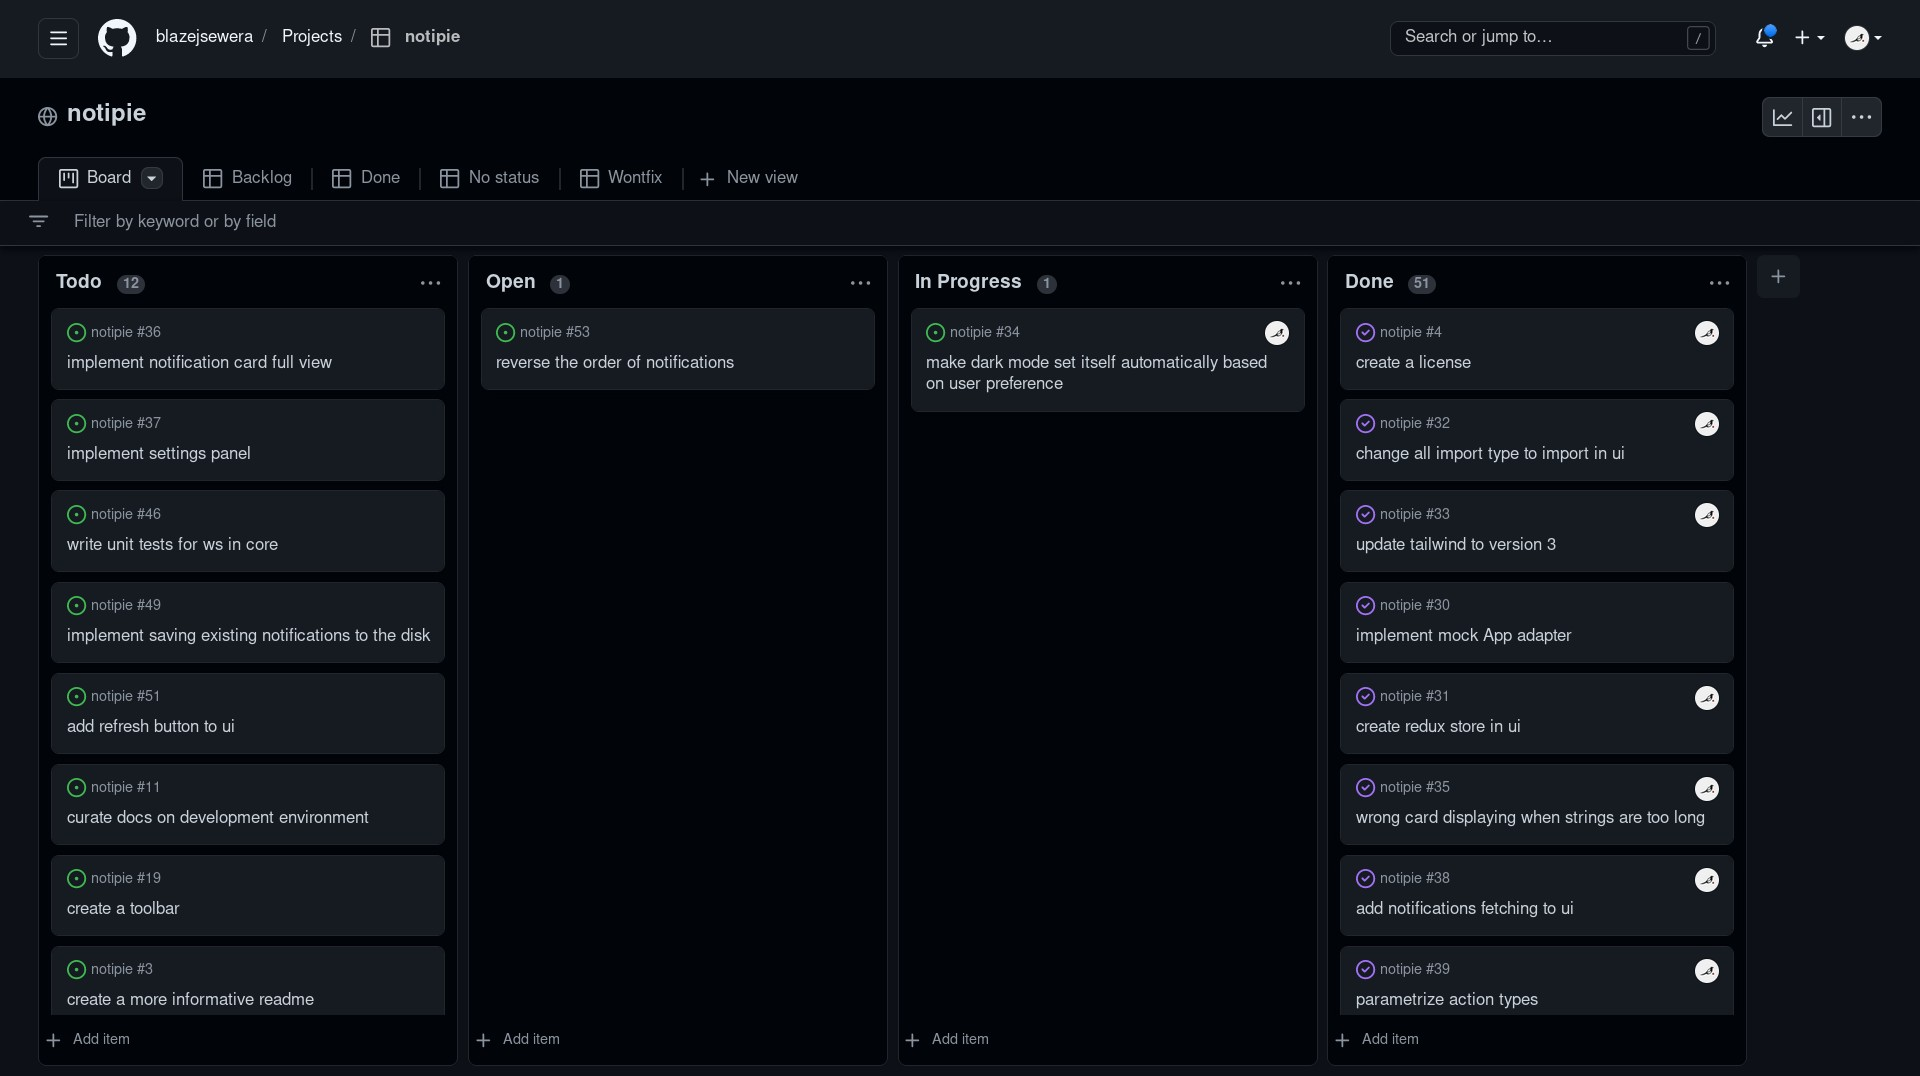
\includegraphics[width=0.99\linewidth,keepaspectratio]{img/kanban_board.jpg}
      \caption{Github Projects: Kanban board view}
      \label{fig:github-projects-kanban}
\end{figure}

\begin{figure}[!h]
      \centering
      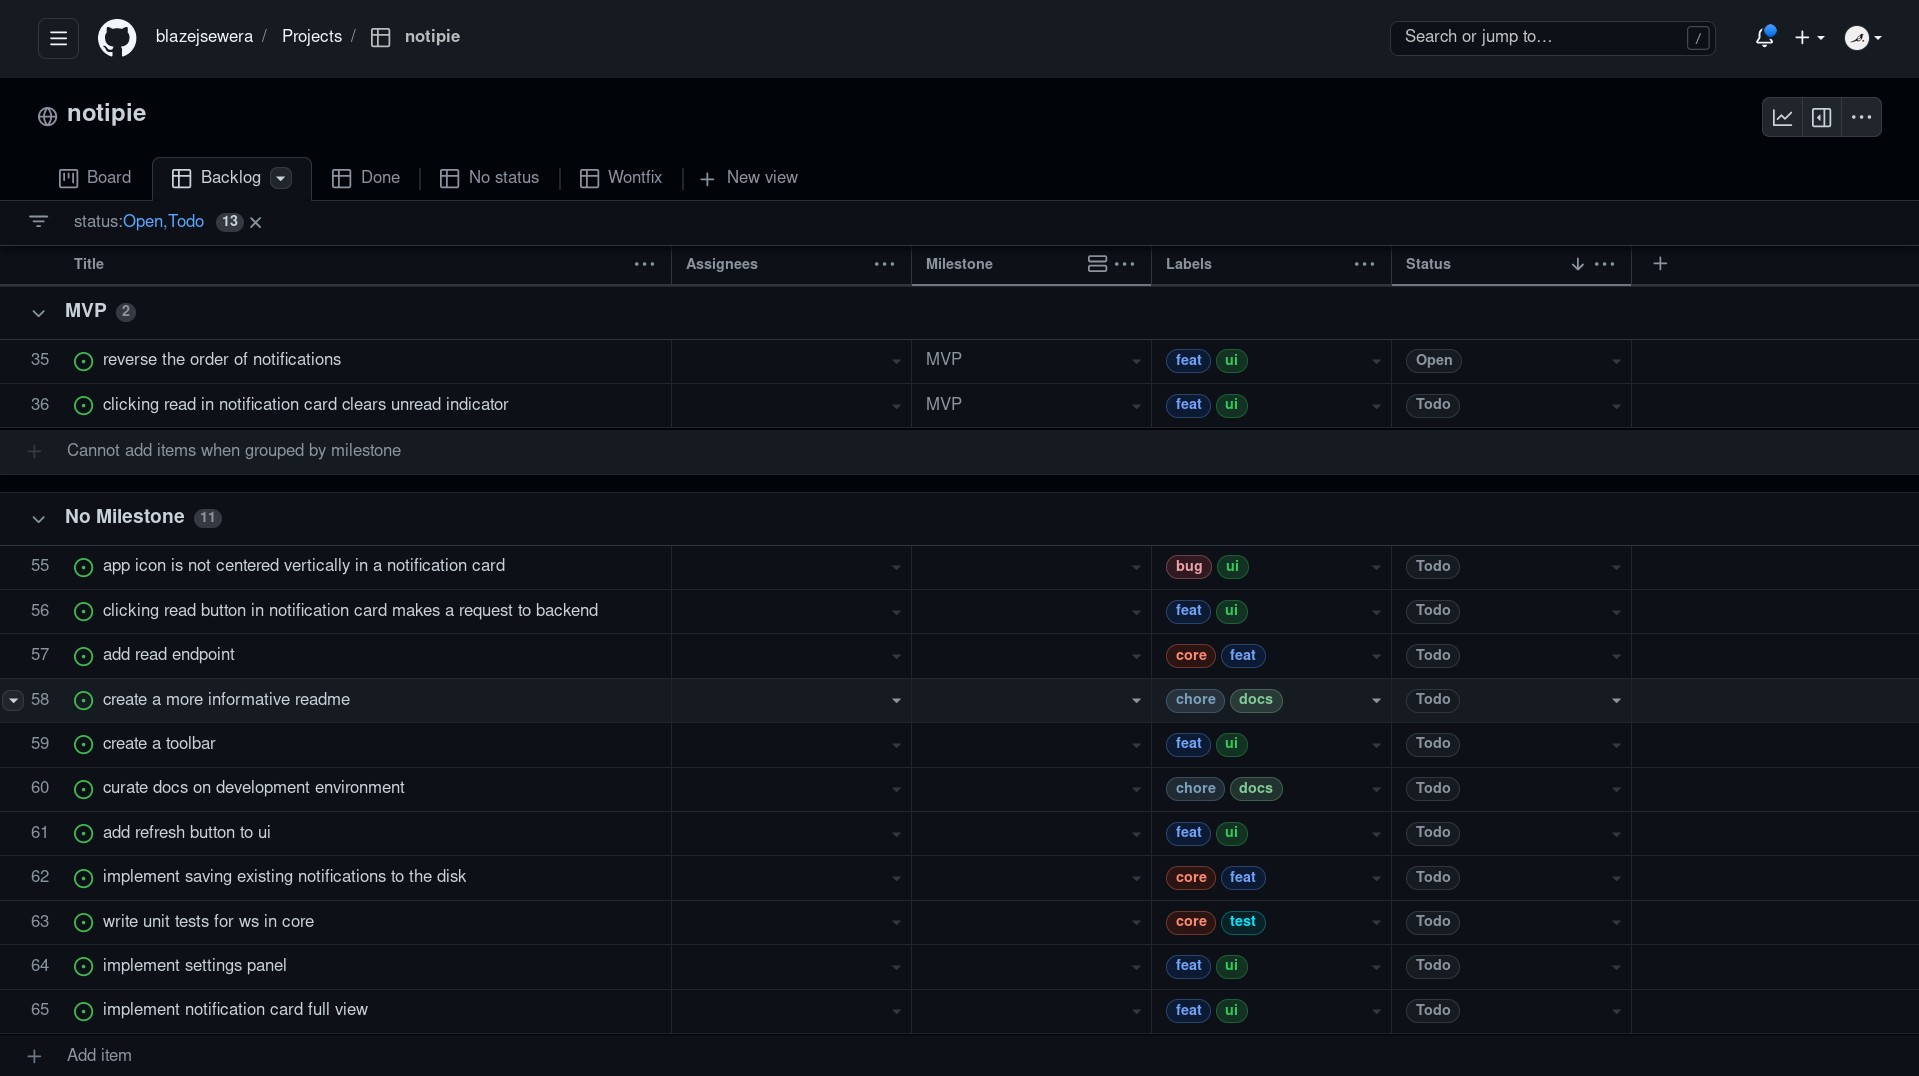
\includegraphics[width=0.99\linewidth,keepaspectratio]{img/backlog.jpg}
      \caption{Github Projects: Backlog view}
      \label{fig:github-projects-backlog}
\end{figure}



\clearpage
\section{Backend}\label{sec:backend}

The backend is a component in a system
that is responsible for the data processing.
It interacts with the frontend applications
with a well-known protocol,
usually one understood by a browser.
Splitting the system into frontend and backend
enables easier reuse of the business logic,
and writing different frontend applications
that use the same backend.
Many huge organizations practice splitting
their systems into frontend and backend.
An example of this is Facebook,
which benefits from the ability to use
many different languages and libraries
that can interact between one another~\cite{abdullah_frontend_2014}.

The backend of Notipie
needed to be both performant,
easy to deploy,
and well-tested.
I strived to make use of the best practices
in the field of microservices,
maintain great quality,
and ensure sufficient performance.
I named it \textit{core},
because there can be different UIs,
or notification producers,
but the entire application's core
is specifically the backend implementation.
The backend code
is in the
\texttt{core} directory~\cite{sewera_notipie_2022}.

\subsection{Core project architecture}\label{sec:core-project-architecture}

An overview of the backend architecture
from the asynchronous notification flow perspective
is presented in figure~\ref{fig:high-level-backend-flow}.
The project on the top-level is structured over 4 directories,
named according to
the \citetitle{quest_standard_2022}~\cite{quest_standard_2022}:

\begin{figure}[h]
      \centering
      \includegraphics[width=6.5cm,keepaspectratio]{chart/out/backend-flow.pdf}
      \caption{Backend architecture for asynchronous notification flow}
      \label{fig:high-level-backend-flow}
\end{figure}

\begin{itemize}
      \item
            \texttt{cmd} -- entry point to the application (\texttt{main})
      \item
            \texttt{internal} -- application-specific code
      \item
            \texttt{pkg} -- reusable utils, not specific to the application
      \item
            \texttt{test} -- black box integration test code
\end{itemize}

\subsubsection{The internal directory}\label{sec:the-internal-directory}

Application-specific code is split into 5 directories
representing the levels of abstraction:

\begin{itemize}
      \item
            \texttt{domain} -- business logic,
            defines data structures and communication of domain objects
            on the highest level of abstraction,
      \item
            \texttt{grid} -- lower level of abstraction than domain,
            defines proxies that convert network models into domain models,
            and connects those proxies with the domain components,
      \item
            \texttt{impl} -- implements network endpoints,
            WebSockets, and persistence,
      \item
            \texttt{infra} -- configures the application
            and sets up the context for DI.
\end{itemize}

There also was a \texttt{model} package
in the \texttt{internal} directory,
but I moved it to an exportable \texttt{pkg} directory,
to reuse it in the notification producer.

\subsubsection{Grid}\label{sec:grid}

The grid is an application layer
that connects implementations of
the endpoints, WebSockets, and persistence
with the domain objects.
I decided to define that name in the UL
to mean this exact intermediate layer.
The name itself was inspired by a power grid
which connects components
from power generation
to appliances.

The implementation is based on the proxies
for domain Apps and Users\footnote{
      The App and the User are defined in
      sections~\ref{sec:app}~and~\ref{sec:user}
      respectively.
}.
Those proxies convert the applicable network models
and perform intermediate procedures
that do not concern the domain,
like Notification ID generation.

This layer is especially important
to keep the domain clean and concise
and to enable easy replacing\footnote{
      The differences between writing code
      for reuse and replacement are described in detail
      in section~\ref{sec:code-quality}.
}
of concrete implementations.

\subsection{Go in core}\label{sec:go-in-core}

Go is quickly gaining popularity among developers,
with its great tooling
and a state-of-the-art standard library.
It is an excellent language for writing microservices.
Its focus on this one task
and pragmatism in adding features to the language by its authors,
resulted in an easy to understand and use,
yet very powerful set of tools.

\subsubsection{Motivation}\label{sec:motivation}

When choosing the right language for the project,
I focused on finding the right tool
for the application and developer experience.

I wanted \texttt{notipie} to be a high-performance microservice,
so I did not take interpreted languages
like Python or JavaScript into consideration.
I mostly considered Java, Kotlin, Rust, and Go.

Java, although popular, does not have the greatest developer experience.
Things like \texttt{equals} and \texttt{hashCode}
are unnecessary bloat in the code.
Project Lombok~\cite{zwitserloot_project_2022} fixes some of them,
but the tooling is limited to IntelliJ,
you have to download a lot of libraries for dealing with JSON,
create your own code style guide,
and perform a fair bit of setup.

Kotlin, far better than Java,
but also locked-in to IntelliJ with tooling,
was an interesting option for me, but not ideal.

Rust was too low-level for my application.
Explicit memory management, although performant,
was simply too verbose and work-intensive for my use case.

Go was a perfect option.
A plethora of great tooling,
like first-party Go plugin for VSCode, GoLand from JetBrains,
community plugins for Neovim,
all working great and providing a good developer experience.
Furthermore, extraordinary performance of the tooling itself,
with tests running in under a second, super-fast compiler,
one of the best standard libraries I have seen,
and overall simplicity of the language, made the choice obvious.

\subsubsection{How did Go make the development easier}\label{sec:how-did-go-make-the-development-easier}

\paragraph*{Built-in language features}\label{par:built-in-language-features}

The features that helped the most during development
were channels and \emph{goroutines},
coroutines automatically managed by the Go runtime.
The idea behind those was very simple to understand,
and working with concurrent programming was a lot easier.

\paragraph*{Goroutines and channels}\label{par:goroutines-and-channels}

Among of the best features of the Go language lay goroutines and channels.
They make concurrent programming a lot easier, compared to other languages.
I used both goroutines and channels
for inter-object communication in \texttt{domain} package.

For example, in {tag.go}~(appendix~\ref{apx:concurrency-in-go}),
after the Tag object is created,
the constructor calls
the \texttt{start} method~(listing~\ref{lst:start-method-in-tag}).
It is running a new goroutine for every Tag instance,
enabling them to asynchronously communicate with other objects.

The Tag was a particularly special case,
in which I had to solve
the Notification duplication problem,
described in detail in section~\ref{sec:tag-technicalities}

\paragraph*{Standard library}\label{par:standard-library}

Standard \texttt{testing} package~\cite{cox_testing_2022} provided
a unified, and simple tooling for testing.
I did not have to think anything about test setup.
No custom scripts, third-party libraries, or IDE setup.
All I needed to do was to name a file with a \texttt{\_test.go} suffix,
write a function starting with \texttt{Test},
and run \texttt{go\ test\ ./...}.
Both VSCode with Go plugin and GoLand
automatically picked up the test setup,
and I was ready to develop with TDD.

Standard \texttt{net/http} package~\cite{cox_http_2022} provides everything
needed for setting up REST endpoints.
Although I used Gin~\cite{martinez-almeida_gin_2022} for this,
due to a simpler interface,
I used status codes and HTTP client implementation from \texttt{net/http}.

\paragraph*{Refactoring to the standards}\label{par:refactoring-to-the-standards}

During this project,
I refactored my functions to better suit
the Go standard library.

For instance,
in commit \texttt{00547cd}\footfullcite{sewera_chorecoreproducer_2022},
I refactored the \texttt{ToJSON} method
to better suit the standard signatures
(appendix~\ref{apx:method-signature-refactoring-in-go}),
i.e. to return the byte array and error,
just like the \texttt{Marshal} method
from the \texttt{json} package~\cite{cox_json_2022}
in the standard library.

\paragraph*{Third-party libraries}\label{par:third-party-libraries}

Gin was great for writing REST endpoints,
with \texttt{gin.Context} having easy access to
standard-library-compatible fields,
making it easily pluggable to other third-party libraries,
like Gorilla WebSocket~\cite{burd_gorilla_2022}.

Zap~\cite{shah_zap_2022} provided a reliable
and performant way to log things in the backend.
Structured logging,
straightforward syntax,
automatic serialization to JSON in production mode,
and human-readable format in debug mode,
paired with low or zero-allocation overhead,
made it a perfect choice for logging in a microservice.

\addtocategory{commit}{sewera_chorecoreproducer_2022}

\subsection{The benefits of using Go}\label{sec:the-benefits-of-using-go}

\subsubsection{Built-in language features}\label{sec:built-in-language-features}

There were numerous features
that helped during backend development.
Implicit encapsulation of functions and variables
starting with a lowercase letter,
structure field annotations
enabling easy serialization
to JSON and YAML,
coroutines automatically managed by the Go runtime,
or channels,
just to name a few.
The idea behind most of them
was very simple to understand,
the usage was intuitive,
and I did not have to resort to the documentation that often.

\subsubsection{Goroutines and channels}\label{sec:goroutines-and-channels}

Among of the best features of the Go language lay goroutines and channels.
They make concurrent programming a lot easier, compared to other languages.
I used both goroutines and channels
for inter-object communication in \texttt{domain} package.

For example, in {tag.go}~(appendix~\ref{apx:concurrency-in-go}),
after the Tag object is created,
the constructor calls
the \texttt{start} method~(listing~\ref{lst:start-method-in-tag}).
It is running a new goroutine for every Tag instance,
enabling them to asynchronously communicate with other objects.

The Tag was a particularly special case,
in which I had to solve
the Notification duplication problem,
described in detail in section~\ref{sec:tag-technicalities}

\subsubsection{Standard library}\label{sec:standard-library}

Standard \texttt{testing} package~\cite{cox_testing_2022} provided
a unified, and simple tooling for testing.
I did not have to think anything about test setup.
No custom scripts, third-party libraries, or IDE setup.
All I needed to do was to name a file with a \texttt{\_test.go} suffix,
write a function starting with \texttt{Test},
and run \texttt{go\ test\ ./...}.
Both VSCode with Go plugin and GoLand
automatically picked up the test setup,
and I was ready to develop with TDD.

Standard \texttt{net/http} package~\cite{cox_http_2022} provides everything
needed for setting up REST endpoints.
Although I used Gin~\cite{martinez-almeida_gin_2022} for this,
due to a simpler interface,
I used status codes and HTTP client implementation from \texttt{net/http}.

\subsubsection{Refactoring to the standards}\label{sec:refactoring-to-the-standards}

During this project,
I refactored my functions to better suit
the Go standard library.
It was beneficial
not only because of a better integration
with the standard library itself,
but also because of a better integration
with third-party libraries.
There is an unwritten rule,
that every library strives
to be as compatible
with the standard library as possible.

For instance,
in commit \texttt{00547cd}\footfullcite{sewera_chorecoreproducer_2022},
I refactored the \texttt{ToJSON} method
to better suit the standard signatures
(appendix~\ref{apx:method-signature-refactoring-in-go}),
i.e. to return the byte array and error,
just like the \texttt{Marshal} method
from the \texttt{json} package~\cite{cox_json_2022}
in the standard library.

\subsubsection{Third-party libraries}\label{sec:third-party-libraries}

Gin was great for writing REST endpoints,
with \texttt{gin.Context} having easy access to
standard-library-compatible fields,
making it easily pluggable to other third-party libraries,
like Gorilla WebSocket~\cite{burd_gorilla_2022}.

Zap~\cite{shah_zap_2022} provided a reliable
and performant way to log things in the backend.
Structured logging,
straightforward syntax,
automatic serialization to JSON in production mode,
and human-readable format in debug mode,
paired with low or zero-allocation overhead,
made it a perfect choice for logging in a microservice.

\addtocategory{commit}{sewera_chorecoreproducer_2022}



\clearpage
\section{Frontend (ui)}\label{sec:frontend-ui}

\subsection{UI Design}\label{sec:ui-design}

When designing the UI of Notipie,
I tried to maximize usability,
and minimize complexity of the interface.
Maintaining simplicity of the interface is not an easy task,
so I took inspiration from the professional designs.

\subsubsection{Inspirations}\label{sec:inspirations}

My main inspirations for the interface were
Apple Human Interface Guidelines~\cite{apple_inc_human_2022}
and Google's Material Design~\cite{google_llc_material_2022},
but by far the most inspiration was taken from
Github Primer~\cite{github_inc_primer_2022}.
I tried to break down what is useful,
what is unnecessary in my project,
and extract only the essentials for my design.

Adam Wathan and Steve Schoger
also had a great influence
on my design decisions.
Their book,
\citetitle{wathan_refactoring_2018}~\cite{wathan_refactoring_2018}
was an excellent guidance of the best practices
of the modern user interface design.

\subsubsection{Final design}\label{sec:final-design}

\paragraph*{The card}\label{par:the-card}

The card is a building block for the entire user interface.
It provides the most interaction in the whole application,
therefore it had to be designed with clearly laid out information
and intuitive controls.
The card itself consists of several elements,
as depicted in figure~\ref{fig:card-with-labeled-elements}:

\begin{enumerate}
      \item
            logo,
            it can be an image
            or automatically generated SVG
            from the first two letters of the app's name,
      \item
            indicator,
            whether the notification has been seen or not,
      \item
            title of the notification,
      \item
            subtitle,
      \item
            body,
            that collapses after it reaches a certain length,
            so that an ellipsis appears (\texttt{...}),
      \item
            information about what app sent the notification and when it happened,
      \item
            controls to archive,
            mark as read,
            or go to external site connected with the notification,
            like a certain build on Jenkins,
            or the notification page on Github.
\end{enumerate}

The card was also designed with aesthetics in mind.
All elements were carefully positioned and aligned,
so they are not only pleasant to look at,
but also have features important for visual communication.
Those features, highlighted in figure~\ref{fig:card-with-guides}, include:

\begin{itemize}
      \item
            the rounded corners take the focus away from the card frame,
            and provide a natural, neutral enclosure for the notification,
      \item
            the inner padding is of equal size in each direction
            to provide optical stability,
      \item
            the distance between the logo and title -- subtitle combo
            is the same size as the padding,
            making the logo appear centered,
      \item
            the title -- subtitle combo itself
            is centered vertically relative to the logo,
      \item
            the distances between the logo,
            notification body, and app name -- timestamp combo are shorter
            in order to make the inner section more connected,
      \item
            the controls are centered relative to the app name -- timestamp combo,
      \item
            the \textit{unread} indicator is unobtrusive enough
            not to steal all the focus from the card's content,
      \item
            finally, the \textit{unread} indicator
            is positioned slightly outside the inner section,
            so that it belongs to the card itself,
            not its content,
            therefore it is easier to spot at a glance.
\end{itemize}

\begin{figure}[p]
      \centering
      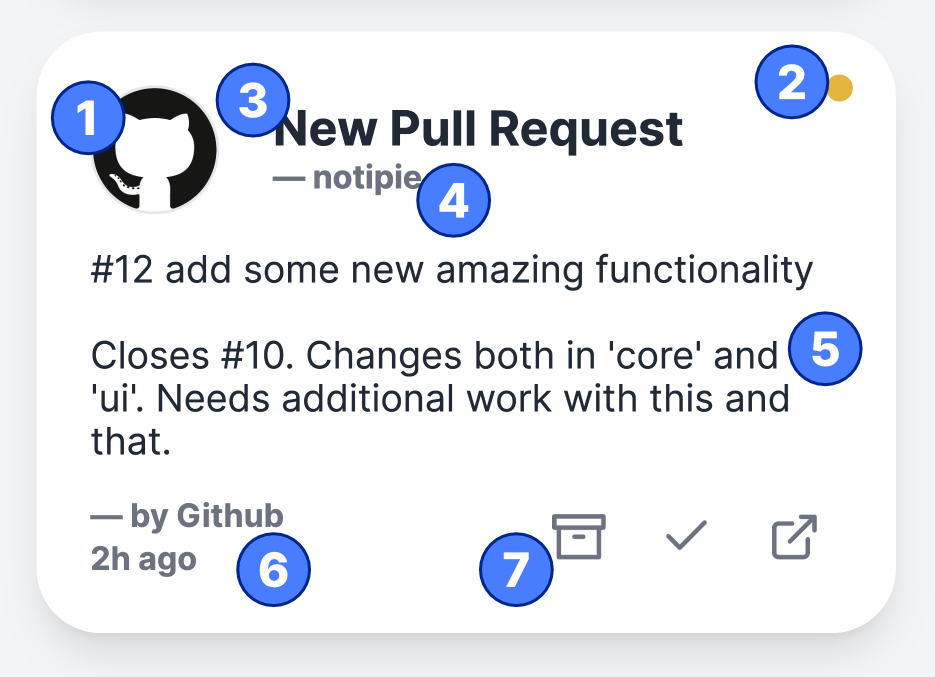
\includegraphics[width=10cm,keepaspectratio]{img/card_labeled.png}
      \caption{The card with labeled elements}
      \label{fig:card-with-labeled-elements}
\end{figure}

\begin{figure}[p]
      \centering
      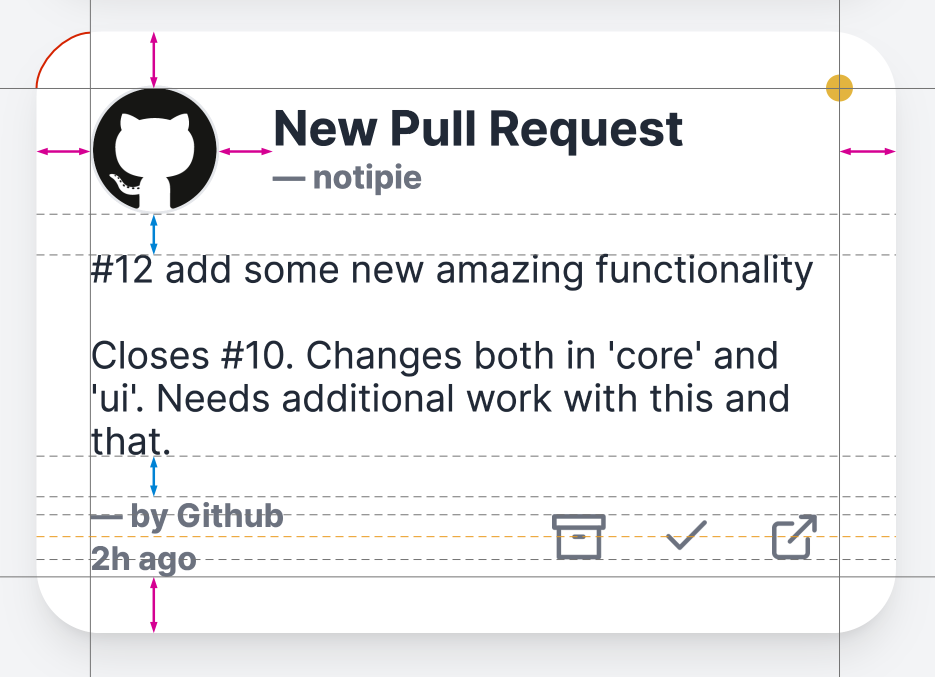
\includegraphics[width=10cm,keepaspectratio]{img/card_guides.png}
      \caption{The card with guides}
      \label{fig:card-with-guides}
\end{figure}

\subsection{UI component library}\label{ui-component-library}

When choosing the library for the UI components, I considered:

\begin{itemize}
  \item
    React\footnote{React, retrieved 2022-05-31. \url{https://reactjs.org/}},
  \item
    Vue.js\footnote{Vue.js, retrieved 2022-05-31. \url{https://vuejs.org/}},
    and
  \item
    Angular\footnote{Angular, retrieved 2022-05-31.
    \url{https://angular.io/}}.
\end{itemize}

All those libraries are very popular, so I chose React, because I had
the most experience with it in my professional work.

\subsection{UI networking}\label{ui-networking}

The nature of notifications required me to use
both REST data fetching and asynchronous data pushes from the backend.
For the latter, I decided to use WebSockets,
a standard defined in RFC6455~\cite{fette_rfc6455_2011}, and
RxJS~\cite{lesh_rxjs_2022}, an implementation of
ReactiveX library~\cite{gross_reactivex_2021}.

\subsubsection{REST data fetching}\label{rest-data-fetching}

I used simple REST~\cite{perrier_rest_2022} requests
for fetching the notifications
that are already on the backend server.
The standard Fetch browser API~\cite{perrier_fetch_2022}
was sufficient for the task.

\subsubsection{Reactive Raven}\label{reactive-raven}

This project~\cite{sewera_reactive_2022} was an experiment
on using RxJS for all real-time data fetching,
enabling the separation of concerns in the code,
and decoupling the state management implementation
from the networking implementation.

When searching for the optimal solution for pushing the data to the UI,
I came across two major solutions:

\begin{itemize}
  \item
        Redux Thunk~\cite{gaeraon_redux_2022-1} --
        enough for fetching data on user interaction,
        e.g., on a button click,
        but it provides virtually full implementation lock-in
        to the Redux store, and very little separation of concerns.
        Fetching data is an action dispatched on a store,
        so external communication and storing data are dependent on each other.
  \item
        Redux Saga~\cite{elouafi_redux_2022} --
        good for managing side effects with plain JavaScript,
        but it uses generator functions
        that yield a different type every time,
        so it is very problematic to use with strict TypeScript.
\end{itemize}

Both thunks and sagas did not provide the separation of concerns
I wanted to achieve.
Fetching or acting upon pushed data
is a different concern than storing it.

As a user,
I should not have to dispatch an action on a store
when I want to fetch data.
Of course, the data can be immediately stored after fetching,
but this behavior should be injected later,
so that there is no store implementation lock-in.

This separation of concerns enabled me to
migrate from Redux to Zustand as my \emph{store} implementation,
as described in the next section.

\subsection{State management in UI}\label{sec:state-management-in-ui}

To simplify the frontend code,
I needed to use a single source of truth for the data.
I used both Redux~\cite{gaeraon_redux_2022},
and Zustand~\cite{kato_zustand_2022} for this task
as \textit{store} implementations,
and Zustand came on top as a simpler solution for my application.

\subsubsection{Redux}\label{sec:redux}

Redux is great for big applications with lots of components.
Being one of the most popular state management libraries for React,
it was my first choice.
Unfortunately,
it required me to write a lot of boilerplate code,
and thus was not easily maintainable
for a smaller project like Notipie.

\subsubsection{Zustand}\label{sec:zustand}

Zustand is a lot simpler than Redux,
requires a lot less boilerplate code,
and was sufficient for my application.
I migrated to it in commit
\texttt{7677d13}\footfullcite{sewera_choreui_2022},
and it reduced the lines of code by over 200.
I did not, however, give up the connected components,
as they provide better testability and separation of concerns,
which is worth a bit extra code.

\addtocategory{commit}{sewera_choreui_2022}

\subsection{TypeScript in UI}\label{sec:typescript-in-ui}

I decided to use TypeScript in my project for the frontend part,
because of its type checking tools,
huge popularity,
and a growing demand for in on the job market.

\subsubsection{Choosing the language}\label{sec:choosing-the-language}

When choosing which language to use in the UI,
I considered a couple of options:

\begin{itemize}
      \item
            plain JavaScript,
      \item
            TypeScript,
      \item
            Elm, and
      \item
            CoffeeScript.
\end{itemize}

I immediately discarded the last two,
due to their smaller popularity,
compared to JavaScript or TypeScript.

The featureset of the language was also very important to me.
JavaScript is by far the most popular,
but it lacks type annotations or pre-runtime type checking.
TypeScript and Elm turned out to be winners in the type checking toolchain.

TypeScript also has a big advantage of being very similar to plain JavaScript,
so the transpiled code is very readable.

A big factor was general trend of language's popularity growth.
TypeScript was a clear winner in this scenario,
being third most loved language
and second most wanted language
in the Stack Overflow Developer Survey 2021~\cite{stack_overflow_2021_2021}.

It was only beaten by Rust and Clojure
in the \textit{Most Loved} section,
both of which are non-frontend languages,
and Python in the \textit{Most Wanted} section,
which is also not a frontend language.

Another report confirming the growing popularity of TypeScript
is Github Octoverse Report 2021~\cite{github_inc_2021_2021}.
Since 2017,
it beat
Ruby,
C,
C++,
C\#,
Shell, and
PHP
and is, as of 2021, the fourth top language on Github.

\subsubsection{Working with TypeScript}\label{sec:working-with-typescript}

Starting with TypeScript was fairly easy.
The toolchain was included in the project creation scripts.
Most dependencies had good TypeScript annotations,
or they were completely written in TypeScript,
which was very helpful for maintaining type safety.

Learning the language was also very easy.
I was already familiar with JavaScript,
so I only needed to learn the type annotations,
which were very intuitive to use.

\subsection{Build system}\label{build-system}

For the build and bundle software,
I wanted to use something modern,
with hot module reloading,
easy to use setup scripts,
customizable development server,
and short bundle times.

\subsubsection{Snowpack and Vite}\label{snowpack-and-vite}

I started with Snowpack~\cite{schott_snowpack_2021}
and used it until I decided to move to Vite~\cite{you_vite_2022}
in commit \texttt{c11bc35}\footnote{
  commit \texttt{c11bc35}, 2021.
    [Online]. (visited on 2022-05-31).
  \url{https://github.com/blazejsewera/notipie/commit/c11bc35370f512f35d522a55fcd216c1c80ea75a}
}.

Snowpack offered both hot module reloading and short bundle times,
however, there were some minor problems from time to time, the project
had a slow development, and the alternative, Vite did not seem to have
those problems.

I tried Vite in my other project, Reactive Raven\footnote{Reactive
  Raven, retrieved 2022-05-31.
  \url{https://github.com/blazejsewera/reactive-raven}}, and the
integration with React, TypeScript, Tailwind CSS, and other tools I used
was seamless, therefore I decided to migrate to it in Notipie as well.

On April 20th, 2022, Snowpack's maintainer stated in the project's
Readme document (commit \texttt{45456aa})\footnote{project's Readme
  document (commit \texttt{45456aa}), retrieved 2022-05-31.
  \url{https://github.com/FredKSchott/snowpack/blob/45456aa14978460afcb5ce20f7296556d22c7595/README.md}}
that they would no longer maintain the project and mentioned Vite as a
good alternative for it.



\clearpage
\section{Producer}\label{sec:producer}

The notification producer for Notipie
needed to be easy to use for developers
and system administrators.
Therefore,
I decided to provide both a Go library,
and a command line utility
that can easily be run on all major platforms
and operating systems.

The notification producer code
is in the
\texttt{producer} directory~\cite{sewera_notipie_2022-4}.

\subsection{Go library}\label{sec:producer-go-library}

In order to make the notification producer
accessible to developers,
I created a simple Go library
for easy notification creation and sending.
The library supports the basic operations
an App\footnote{
  The App is defined in section~\ref{sec:app}.
} can perform.

Those operations include pinging the backend if it is up
and pushing the notification to the backend.

The first operation is useful when setting up
a producer that can push to different backends,
depending on which one is up.
For example,
two backends are running
in two different VPNs.
Depending on which one of them
the computer producing notifications
is connected to,
it first pings those two,
and decides on which one to send the notification to.
This operation can be performed
when starting the producer up,
without the need to send a real notification.

Pushing the notification to the backend
also includes getting the App ID from the backend.

\subsection{Command line utility}\label{sec:command-line-utility}

Not everyone who could benefit
from my application
needs to have a good understanding
of Go development.
That is why I also prepared
a command line utility
that is compatible with the most popular shells:
Unix-like shells and Powershell.

Its feature set is very similar
to the one mentioned in the previous section,
but it also includes configuration
and notification templates
for convenience.
This in turn enables its users
to set up the producer for multiple Apps
on one system.
It is only necessary to provide
separate configuration files
and, optionally, separate notification templates.
An example of such setup is presented
in figures~\ref{fig:notipie-one-notification}
and~\ref{fig:notipie-two-notifications}.

\subsubsection{Configuration and notification templates}\label{sec:configuration-and-notification-templates}

This version of a producer can be configured
either through the command line arguments,
or the configuration files,
but the command line arguments
always take precedence.
The configuration files themselves
can be stored in \ac{JSON} or \ac{YAML} format.
I chose those two,
because they are very popular formats
for this use case.
Those formats can also be used
for specifying a notification template.

The configuration consists of
the address and port of the backend,
which are set by user.
Also, when the producer sends its first notification
and gets back the App \ac{ID},
the producer appends it to the configuration file,
so that it is present in every consecutive push.

The notification template can be any
subset of an App notification model
defined in section~\ref{sec:protocol}.
Everything specified in this template
can be overwritten with \ac{CLI} arguments.
The only requirement for a valid request
is to have an App name and title set.
The timestamp is set automatically for us.

\subsubsection{Usage}\label{sec:producer-usage}

As described in the previous section,
the producer allows different configurations
for one \ac{CLI} program,
enabling user to set up many different Apps
on the same computer.
Figures~\ref{fig:notipie-one-notification}
and~\ref{fig:notipie-two-notifications}
show the producer sending the notifications
to the Notipie \ac{UI}.
The producer is executed
with different configurations
and notification templates.
The configurations only differ
with the randomly-generated App \ac{ID}.

\begin{figure}[p]
  \centering
  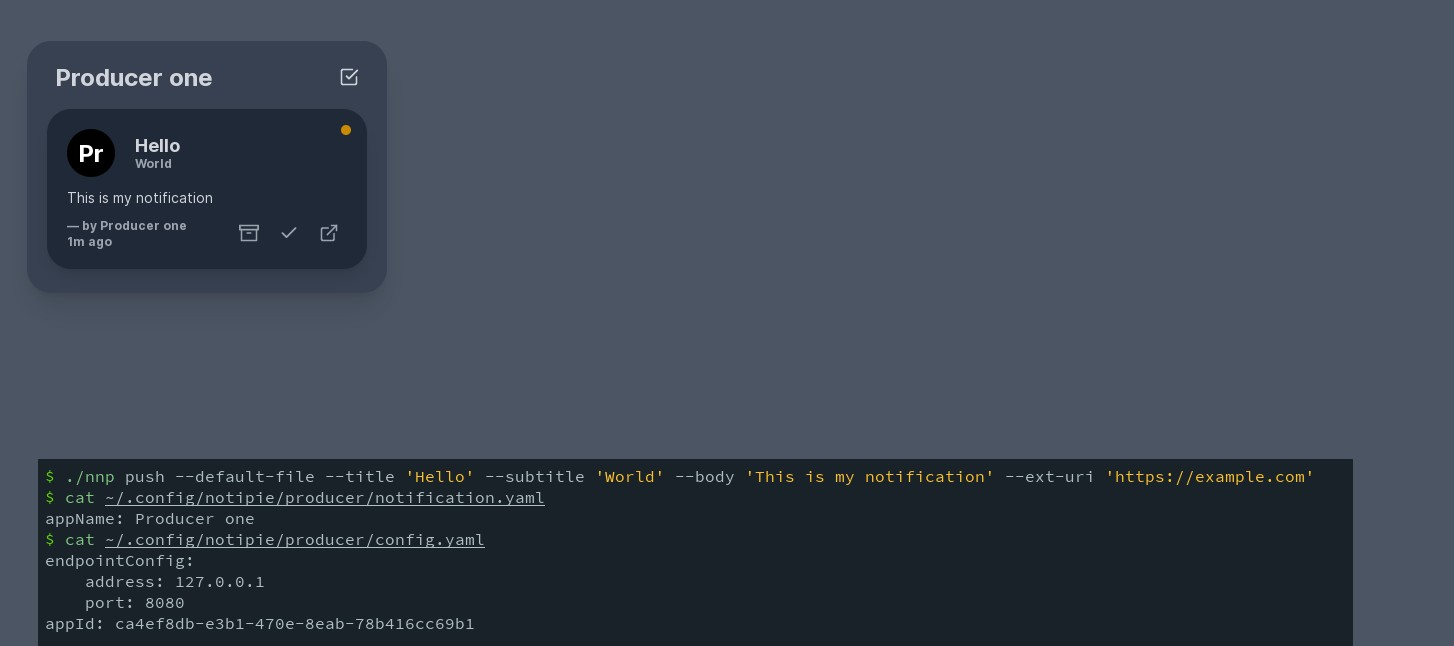
\includegraphics[width=\linewidth,keepaspectratio]{img/notipie_one_notification.jpg}
  \caption{First producer pushing a notification to the UI}
  \label{fig:notipie-one-notification}
\end{figure}

\begin{figure}[p]
  \centering
  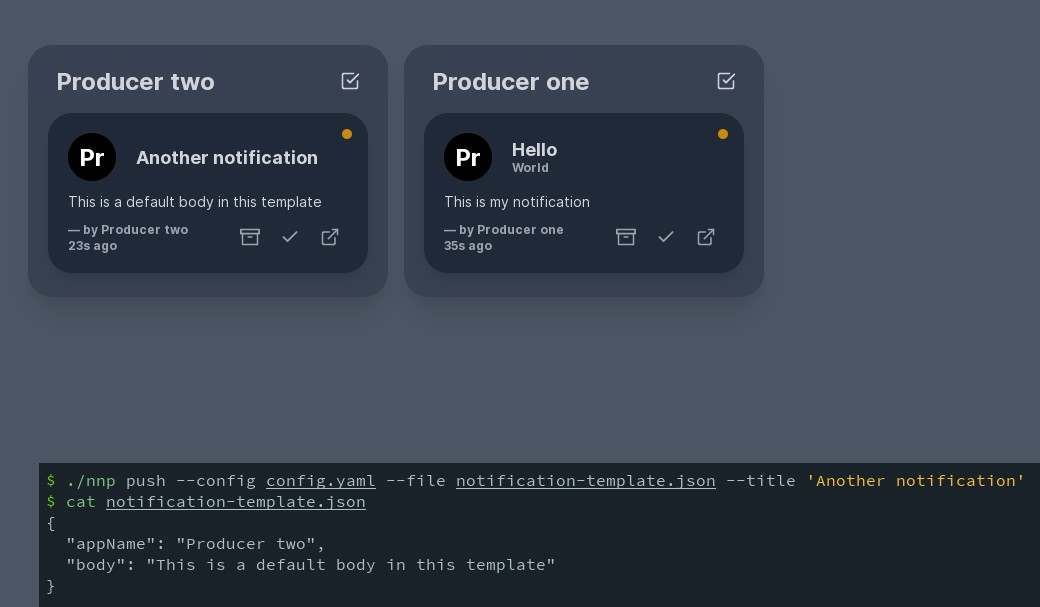
\includegraphics[width=\linewidth,keepaspectratio]{img/notipie_two_notifications.jpg}
  \caption{Second producer pushing a notification to the UI}
  \label{fig:notipie-two-notifications}
\end{figure}



\clearpage
\section{Protocol}\label{sec:protocol}

The Notification\footnote{
  The Notification is defined in section~\ref{sec:notification}.
} in the terms of a domain
was not suitable for the communication
between the producer, backend, and frontend.
That is why I specified a network protocol
for sending notifications
and replying with App ID to a producer.
I needed to choose the right format
and develop a set of fields
containing all the useful information.

\subsection{Format}\label{sec:protocol-format}

When I was choosing the right format
for the notifications,
I took into consideration two options:
binary and plain text.
I chose plain text,
because portability was very important to me.
I wanted to have the protocol able to run
between different processor architectures,
and not think about endianness.

Then, I wanted to use a format
that was popular for network data exchange.
The candidates were XML and JSON.
I did not want to go with XML,
as the parsing is not that easy,
readability is very poor,
and the popularity is dropping
in favor of JSON.
I chose JSON,
because of its support by TypeScript and Go,
either as a language feature,
or in a standard library.
I also chose JSON for the push response
containing App ID
for consistency.

I decided to support both JSON and YAML
in the configuration files for the producer,
including the notification template\footnote{
  More on the configuration files and templates
  for the producer
  in section\ref{sec:configuration-and-notification-templates}.
}.
YAML is favorable in configuration files,
so I wanted to provide a uniform
format for a configuration file
and a template.
YAML, however,
does not go through the network
anywhere in Notipie.

\subsection{Fields}\label{sec:protocol-fields}



\clearpage
\section{Programming Practices}\label{sec:programming-practices}

Programming is a very complex activity
in which an error can cause a hard to find bug
or prevent compilation altogether,
which in turn slows the development down.
To mitigate the risks of human error,
I used numerous programming practices
taken from \ac{XP}~\cite{beck_extreme_2004},
as well as personal and professional experience.

\subsection{Test-driven Development}\label{sec:test-driven-development}

For the development of the domain,
I used all the best practices I knew.
One of them was test-driven development.
I read about \ac{TDD} multiple times, in
\citetitle{beck_test-driven_2002}~\cite{beck_test-driven_2002},
\citetitle{martin_clean_2011}~\cite{martin_clean_2011}, and
\citetitle{beck_extreme_2004}~\cite{beck_extreme_2004}.

I followed the red, green, refactor cycle,
checking every time that I understand
the usage of the code I wrote.
It enabled me to have an architecture
in the domain package I am proud of,
without a huge effort.

I only regret that
I did not fully commit to the test-first development.
The \texttt{impl} and \texttt{infra} packages
are not well-tested,
and I even resorted to copying the example implementations
from the Gorilla WebSocket~\cite{burd_gorilla_2022} documentation.
It turned out to be a bad idea,
when I encountered hard to spot bugs,
like the one
where the \ac{WS} server
was pinging a disconnected client,
resolved in commit \texttt{fc34a8b}~\footfullcite{sewera_fix_2022}.

\addtocategory{commit}{sewera_fix_2022}

\subsection{Continuous Integration}\label{sec:continuous-integration}

Following \ac{XP} practices,
I acknowledged the need for
continuous builds of my application~\cite[pp.~49-50]{beck_extreme_2004},
so I decided to create a \ac{CI} pipeline.
I went with Github Actions~\cite{github_inc_github_2022-1},
because I have already had
the code repository in Github,
and it was easy to set up.

I also knew it has to satisfy
the ten-minute build constraint~\cite[p.~49]{beck_extreme_2004},
so I constantly made little changes
to make the build performant.
The biggest change to improve
the build time was to use caching.
For this task, I chose a first-party library,
Actions/Cache~\cite{sharma_actionscache_2022}
due to its integration with Github Actions.
I managed to optimize the build
from about 3.5 minutes
in the Notipie \ac{CI} run number 116~\footfullcite{sewera_notipie_2022-1}
to only 2 minutes after caching
in the run number 118~\footfullcite{sewera_notipie_2022-2}.

\addtocategory{commit}{sewera_notipie_2022-1,sewera_notipie_2022-2}

\subsection{Git hooks}\label{sec:git-hooks}

Git hooks are a great tool
for enforcing common style guidelines,
commit message format,
and as a general reminder
to perform certain tasks before checking in the code.
They are shell scripts ran by Git
when certain events occur.
I use pre-commit and commit-msg hooks.
A pre-commit hook runs just before committing
and prevents a commit if it fails.
A commit-msg hook simply checks
if a commit message written by a programmer
meets certain criteria.

From my professional experience,
git hooks have to be very quick,
preferably almost instant,
otherwise they will be skipped
with a \texttt{{-}{-}no-verify} flag.
At the beginning,
I have set up git hooks
with Husky~\cite{typicode_husky_2022},
but being written in \ac{JS},
they sometimes ran for over half a minute.
I decided to go with manually written shell scripts
as git hooks.
They turned out to be very performant,
easy to set up, and customize.
For a pre-commit hook I set up code formatting checks.
If the staged for commit code is not formatted correctly,
it fails.
For a commit-msg hook I set up a regular-expression-based
message checking.
The commit message has to follow
Conventional Commits Specification~\cite{petrungaro_conventional_2019}.

\subsection{Build automation}\label{sec:build-automation}

A build system is a program or set of programs
that automates commonly-used actions.
It dramatically speeds up the development cycle,
reduces manual repetition of the tasks,
and in turn,
reduces the number of possible mistakes
that could be made had those tasks
been performed by hand.
Those actions include:
\begin{itemize}
  \item dependency synchronization,
  \item project compilation,
  \item project testing,
  \item starting a development environment,
  \item creating Docker images,
  \item and more.
\end{itemize}

When developing the application,
it is very important to automate the build process.
For this task,
I chose \texttt{package.json} scripts
for \ac{TS} projects,
and Make for everything else.

It was very important for me
to have this project ready for development
after running only one script.
That is why I prepared a Make recipe
which guides a user on how to install
Go, Node.js, and Yarn,
which installation could not be automated,
and installs the prerequisites for all components.
It also copies example configuration files
to the necessary places,
and installs Git hooks,
so that a full local development setup
is configured.

I also provided many recipes
for configuration files management,
building binaries,
Docker images creation,
quick application running with hot reload,
testing,
linting, and
code formatting
to further speed up the tasks
that developers do repeatedly.

I chose to use \texttt{package.json} scripts
for \ac{TS} projects,
because they are widely used
across the frontend developers,
and there is a better chance
that when someone wants to contribute
only to the frontend project,
they will be more familiar with those scripts
than with Make.

\subsection{Containerization}\label{sec:containerization}

% TODO: Elaborate (eng-thesis #22)
Containerization is a technique of running an application
in a virtualized environment.
A container provides all the necessary dependencies
for the application,
for instance, shared libraries,
like \texttt{libc} and core utils implementations.
There is a difference between container-based virtualization
(containerization) and full virtualization, though.
The container runs on a shared kernel,
as opposed to having its own
virtual CPU, memory, and own kernel~\cite{watada_emerging_2019}.
The main advantage is to maintain separation
and minimize coupling between
the major components of the architecture~\cite{stytz_rapid_1997},
most often microservices.

I decided to use the Docker technology
for containerization in my project.
Not only is it a good fit for microservices,
but also it features many time-savers in its ecosystem.
For example,
defining containers
is as easy as writing a Dockerfile.
The public Docker Registry,
called Docker Hub contains a plethora
of useful existing images ready for use~\cite{jaramillo_leveraging_2016}
that include, inter alia:
Linux distributions, like Debian,
reverse proxies, like Nginx,
or build environments, like Node.js.

To simplify the deployment process,
I decided to containerize my application
with Docker.
For the backend container,
I used different images
for building the binaries
and for running the service.
For the frontend container the approach was similar,
but for generating static files
and hosting them.
The setup is depicted in appendix~\ref{apx:containerization-with-docker}.

\subsection{Monorepo}\label{sec:monorepo}

Monorepo is just a single repository
for the whole solution.
All the components are in one repository,
including frontend,
backend,
producer, and
testing tools.
It greatly improved and simplified
the integration between frontend, backend,
and gave way for scripts
bringing the whole stack up.
The unit and integration tests run for all
components simultaneously,
so that if something in the product breaks,
it is immediately visible.
I can take full advantage of the
``stop the presses'' \ac{CI} pipeline failure approach,
explained in \citetitle{martin_clean_2011}~\cite{martin_clean_2011}.

Not only that,
but it also simplified sharing
the common protocol models (section~\ref{sec:protocol})
for the Go projects, i.e. backend and producer,
without the need for additional procedures
for releasing the libraries with models.

Such monorepos provide many advantages
when keeping the whole product in one place.
Refactoring,
even a full-stack-wide
is very easy in such a repository,
and can be brought down to a single \ac{PR}.
This in turn decreases the lag between
opening a \ac{PR} and merging it,
compared to many \acp{PR} in many different repositories.
It is especially important
to optimize the \ac{PR} times in open-source,
because here we cannot avoid them,
in contrast to the \ac{XP} teams~\cite{beck_extreme_2004},
in which the only contributors are its members.



\clearpage
\section{Domain}\label{sec:domain}

\Ac{DDD} is a software design approach
that aligns the code with the reality
of the problem domain.
It achieves said alignment by focusing
on the following components of the problem domain:
its terminology,
the core reasons behind why the software is being developed,
and success definition.
Because of this alignment,
adding new features is easy,
and the understanding of the problem domain
stays in sync with the production code~\cite{millett_patterns_2015}.
A model of the solution is called the domain model.
The production code needs to directly reflect the domain model,
which means that \iac{UL}, a set of definitions
understandable both to domain experts
and to developers~\cite{evans_domain-driven_2003,millett_patterns_2015},
has to be defined.
\Ac{UL} helps with confronting the proposed solutions
between these two groups.

I started tackling the problem domain by
laying out the high-level definitions
of all significant parts
that are necessary to implement the solution.
I wanted the domain of my application
to be as simple and clear as possible.
Therefore,
I came up with \iac{UL}
and defined four main components: Notification, Tag, App, and User.

\subsection{Notification}\label{sec:notification}

The core of the application.
This is the structure
acting as a protocol of communication
between all components in the application domain.
It consists of the text fields,
like title, optional subtitle, optional body,
\acp{URI} for marking the Notification read,
but also an App\footnote{
  The app component is explained in detail in section~\ref{sec:app}
} of origin.

For the distributed nature of the components,
the Notification is always passed by value.
Having an immutable copy of the Notification object
in every place ensures
no unexpected states in the application.
It is easily achieved
using the features of
the Go language\footnote{
  More on Go features in section~\ref{sec:the-benefits-of-using-go}
}.

\subsection{Tag}\label{sec:tag}

The Tag in the Notipie domain
is a Notification broker
between the Apps and the Users.
It stores which Apps are attached
and which Users are subscribed to it.
It also ensures thread-safety
for attaching and detaching of Apps,
as well as subscribing and unsubscribing of Users.

At first,
I wanted it to be named ``Room'',
like a chat room,
so that many Users could have been
in different Rooms,
similar to subscribing to multiple Tags.
However,
it was less understood by people I spoke with,
mainly due to the fact,
that one App sending to different rooms,
and a User being in different rooms simultaneously,
contradicts the existing understanding of chat rooms.

A User can subscribe to the Tag,
and an App can add itself to a Tag.
When that happens,
the forwarding of Notifications
between said App and User is enabled.
Thread-safety of those operations
are ensured by mutexes\footnote{
  A mutual exclusion lock.
  A mutex serializes the execution
  of multiple threads~\cite{mattson_patterns_2004}.
}.
The Tag is actively listening
on the Notification channel (\texttt{NotificationChan}),
and every time a new Notification arrives,
the \texttt{broadcast} method~(listing~\ref{lst:broadcast-method-in-tag})
is executed.
The \texttt{broadcast} method then sends that Notification
to every User subscribed to this Tag.
The flow is presented in figure~\ref{fig:notification-flowchart}.

\begin{figure}[h]
  \centering
  \includegraphics[width=10cm,keepaspectratio]{chart/out/notification-flowchart.pdf}
  \caption{Notification flow in \texttt{domain}}
  \label{fig:notification-flowchart}
\end{figure}

\subsubsection{Technicalities}\label{sec:tag-technicalities}

There is an obvious problem with this approach.
When a User is subscribed to two Tags,
and one App has those two Tags assigned,
then that User can get the same Notification twice
(figure~\ref{fig:duplicated-notification}).
There are two solutions I could think of.

\begin{figure}[h]
  \centering
  \includegraphics[width=10cm,keepaspectratio]{chart/out/duplicated-notification.pdf}
  \caption{Duplicated Notification flow}
  \label{fig:duplicated-notification}
\end{figure}

\paragraph*{Solution 1}\label{par:duplication-solution-1}

This solution assumes the following:

There is a new component in the domain, Router.
It is a centralized component
that knows which App is connected to which Tag,
and which User is subscribed to those Tags
(figure~\ref{fig:notification-router}).

\begin{figure}[h]
  \centering
  \includegraphics[width=15.5cm,keepaspectratio]{chart/out/notification-router.pdf}
  \caption{Notification Router}
  \label{fig:notification-router}
\end{figure}

With this approach,
the User component is simpler,
as it does not need any deduplication logic.
However, there is a whole new component
in the domain, which introduces complexity.
Furthermore, the Router has to be
a Singleton~\cite{gamma_design_1994}
in order to process all the Notifications.
It would create a bottleneck,
as the Router would need to process every new Notification
that goes through the application.

The Router needs a table referencing
Tags and Users subscribed to them.
Provided that there are $n$ Tags,
and every Tag has $m$ Users subscribed to it,
the lookup complexity of such table
would be $O(n \cdot m)$,
because the table would need to be
scanned in its entirety to determine
all the Users that need to get the Notification.
It could be optimized into $O(m \cdot \log n)$
if the Tag list is sorted,
but the sorting would introduce
more complexity in the Router.

The time complexity was not the main concern, though.
Martin Fowler insisted on doing performance optimizations
after taking care of code complexity~\cite{fowler_refactoring_2019},
so my main concern was additional code complexity,
compared to the second solution.

\paragraph*{Solution 2}\label{par:duplication-solution-2}

This solution assumes the following:

The deduplication logic is inside the User,
every Notification is sent by a Tag to a User
if the User is subscribed to the Tag.
The User decides if it keeps the Notification
or drops it as a duplicate
(figure~\ref{fig:notification-user-dedupe}).

\begin{figure}[h]
  \centering
  \includegraphics[width=15.5cm,keepaspectratio]{chart/out/notification-user-dedupe.pdf}
  \caption{Notification Deduplication in User}
  \label{fig:notification-user-dedupe}
\end{figure}

With this approach,
the User component is more complex,
but the overall domain structure is simpler.
The Users are distributed across the application,
and only need to deduplicate their own Notifications.

The solution is parallelized by nature,
so there is no bottleneck
like with the previous example.
The solution is also more scalable.
As the application grows,
and more Notifications go through it,
we can start to observe race conditions.
In result,
duplicated messages from different Tags
will start to appear.

Then, we can simply extend the length of
previous Notification \acp{ID} that we check.
We can start with keeping as many previous
Notification \acp{ID}
as there are Tags the User is subscribed to.
The code complexity is also superior
to the previous approach.
Dropping or saving a Notification is a trivial task,
with a simple algorithm:
when the current Notification \ac{ID} is found in the
already received \acp{ID}, drop it; otherwise, save it.

\subsection{App}\label{sec:app}

The App is able to send Notifications
in the domain.
Conceptually,
there is one instance of an App
per each real application
able to produce notifications.
Multiple Apps per one producer scenario
is explained in detail in section~\ref{sec:producer-usage}.

For instance,
when I set up a health checking script
that produces a notification each time
a Systemd service is started,
like the one in listing~\ref{lst:sample-systemd-service-definition},
when any of the hooks fire,
and the notification arrives to the backend,
a new App is created in the domain.
When this happens,
a new App ID is generated
and is later sent back to the producer.

\subsection{User}\label{sec:user}

The User is a recipient of the Notifications.
Whenever a Notification
goes through the Tag a User is subscribed to,
they get this Notification.
The User is also responsible for
the deduplication of the Notifications,
should they arrive from multiple different Tags.
It is explained in detail in section~\ref{sec:tag-technicalities}.



\clearpage
\section{Quality}\label{sec:quality}

I want to take pride in what I do.
Therefore,
I took extra care when I created Notipie
to account for the quality of the product.
I defined the quality as follows:

\begin{quote}
  \begin{enumerate}
    \item Sufficient product success,
    \item Sufficient product reliability, and
    \item Sufficient product maintainability and developer satisfaction.
  \end{enumerate}
\end{quote}

I also defined success as:

\begin{quote}
  \begin{enumerate}
    \item Sufficient correctness of the delivered information,
    \item Sufficient usefulness of the delivered information, and
    \item Clear presentation of the information.
  \end{enumerate}
\end{quote}

I did not define success in the commercial terms,
because that was not the scope of my project.
I managed to keep my focus on quality,
and keep the list of features in check
by defining an \ac{MVP}.
I also double-checked the correct behavior
of my application with manual \ac{E2E} tests.

\subsection{Minimum Viable Product}\label{sec:minimum-viable-product}

Eric Ries described the role of the \ac{MVP}
as a reliable feedback of an idea~\cite{ries_lean_2011}.
Agile Alliance stressed the need
for the quality of that product~\cite{foster_mvp_2022}.
William S. Junk characterized the balance between
a schedule,
resources,
product features,
and quality~\cite{junk_dynamic_2000}.

I knew good quality not only is a requirement
to present the application to the potential users,
but also it reduces stress,
allows me to progress as a professional,
be proud of the work I do,
and prepare for the eventual extension
of the application~\cite{beck_extreme_2004,foster_mvp_2022,martin_clean_2011}.
I wanted my solution to be
as bug-free as possible.

Because of my limited schedule,
resources limited to only one programmer,
and the need for quality,
I did not want to incorporate
any excessive features.
The~\acl{MVP} definition is as follows~\cite{sewera_mvp_2022}:

\begin{itemize}
  \item Notifications can be sent with a manually programmed script
        with the help of a library.
  \item They arrive to the \ac{UI} in real time.
  \item The library is provided in the \ac{MVP}.
  \item The backend correctly forwards those notifications to the frontend.
  \item The backend stores existing notifications in memory.
  \item The frontend correctly presents notifications to the user.
\end{itemize}

\subsection{E2E Testing}\label{sec:e2e-testing}

There are two ways of E2E testing,
manual and automatic.
I chose the former,
because writing automatic tests
require a complex setup,
a new framework like Selenium~\cite{steward_selenium_2022},
and a whole other project to maintain.
E2E test automation is of substantial advantage
for bigger projects, however,
my project is well tested with
unit tests,
integration tests, and
snapshot tests\footnote{
  Snapshot testing is a frontend-specific term
  explained in section~\ref{sec:ui-testing}.
}.
All of those automatic tests
raised my confidence in the project high enough
that I did not have to manually test
the application very often.

Despite that,
I created two manual testing utilities,
which helped me with development
of frontend and backend components independently,
a test notifications server
and a test WebSocket client.
I chose to write both of them in TypeScript,
with as little code as possible;
first not to introduce another language
to the project, like Python,
and second to reduce the overhead
of a statically-typed language
for such a simple, non-critical task.

\subsubsection{Test Notifications Server}\label{sec:test-notifications-server}

The test notifications server
is a very simple server that sends
randomly-generated notifications to the UI.
It can send an initial batch of notifications
when the UI calls the endpoint synchronously,
but it also can accept a WS connection
and send one notification at a time asynchronously,
on a press of the \textit{Enter} key.

The server itself is written
using Express~\cite{holowaychuck_express_2022},
a lightweight HTTP framework.
The random notification generation
is done with a help of Faker~\cite{marak_faker_2022},
a JS library for generating fake,
but realistically-looking data.

I used it for checking if the UI
is wired up properly,
when I did not have
the notification producer
implementation in place.

\subsubsection{Test WebSocket Client}\label{sec:test-ws-client}

The test WS client
is a simple client that connects
to a hard-coded URL on start,
sets up the WS connection,
and logs everything that is pushed to it.
It also closes the connection before stopping.

For the implementation,
I used the built-in standard WS implementation
in Node~\cite{trott_node_2022}.

I used this test client
to check if the backend properly
sets up the connection,
creates the client object,
sends the data,
and destroys the object properly
after the client disconnects.

\subsection{Code quality}\label{sec:code-quality}

Apart from the quality of the product,
or rather in concert with it
comes the code quality.
I spent a fair amount of time trying
to perfect maintainability,
scalability,
and reusability of the code.
One big thing that helped me with this task
was test-first development,
explained many times by Kent Beck or
Robert C. Martin~\cite{beck_extreme_2004,beck_test-driven_2002,martin_clean_2011}.
I cannot stress enough how big
of a change in development pace it brought.
Another thing was refactoring,
explained in detail,
with a handy glossary,
by Martin Fowler~\cite{fowler_refactoring_2019}.
Together with \ac{XP}~\cite{beck_extreme_2004},
it ensured me that designing the architecture right
the first time rarely works.

\citetitle{millett_patterns_2015}~\cite{millett_patterns_2015}
and \citetitle{evans_domain-driven_2003}~\cite{evans_domain-driven_2003}
showed me a different perspective
of not getting something right the first time,
but this time it was specifically the domain.
For instance,
I struggled a lot with the Tag definition,
name, and set of responsibilities.
The informal discussions with my friends
helped me gain additional insight into the domain
from a different point of view.

Those two books also broke down the intricacies
of writing the code for reuse or replacement.
I could, for example,
migrate pretty easily
from one state management implementation to another,
as described in section~\ref{sec:state-management-in-ui}.
I can also easily swap
the persistence implementation in the backend,
from in-memory to a proper database.



\clearpage
\section{Takeaways}\label{sec:takeaways}

The main goal of this project
was to learn as much as possible about
frontend and backend development,
testing,
\ac{UI} design, and
project management,
as well as grow as a professional,
evaluate best practices,
and gain experience.
I am proud of what I did right,
and satisfied with the lessons
I have got from what I did wrong.

\subsection{What went right}\label{sec:what-went-right}

I am happy that I have set up a \ac{CI} pipeline
in Github Actions~\cite{github_inc_github_2022-1}
pretty early in the project,
before I even acknowledged how important it is
when reading Kent Beck's book on \ac{XP}~\cite{beck_extreme_2004}.
It significantly sped up my development cycle,
and~provided me with invaluable feedback,
even when I pushed the code to the server
and turned off my computer.
The \ac{CI} pipeline, however,
would be of no use had I not written
any automated tests.
The most comprehensive test suite,
which checks the most crucial paths
in backend,
was the integration test suite,
listed in appendix~\ref{apx:integration-test-core}.

As I was writing the core domain code,
I followed another Kent Beck's advice,
and I left breaking tests between commits.
It was an advice for single-developer projects
utilizing \ac{TDD}~\cite{beck_test-driven_2002}.
When there are at least two developers,
it is much easier to keep track of what is going on.
When I get distracted,
I lose focus and current context of the code.
In pair programming,
the second programmer can take over this context
and maintain continuity.
In a single-developer project,
the~foregoing failing tests act as a second programmer
in this regard,
and they mark a clear place
to take up where I left off.

I am very proud of my experiments
on the code,
like Reactive Raven~\cite{sewera_reactive_2022},
explained in section~\ref{sec:reactive-raven},
or connecting snapshot testing
with a \ac{CSS} utility library
to avoid slow visual tests,
which is explained in section~\ref{sec:ui-testing}.

Not including a database in the \ac{MVP}
was also the right choice.
I noticed in my professional career that
deciding which database is right for the application early on,
usually produces a lot of problems.
For instance,
if chosen database has insufficient performance,
the work needed for that database setup is wasted.
On~the other hand,
when we choose a database tailored for performance,
we might need to handle a more complex setup.
If our application turns out to be of low throughput,
said more complex setup and additional maintenance
is also wasted time,
as a simpler one would suffice.
We should postpone the decisions as far as we can,
because only then we have the most information
and knowledge to make one~\cite{erder_principle_2016}.
So it was not dictated
by my reluctancy to add one,
but rather an informed decision
to first measure the real-world traffic
in my application,
and then add a proper database,
based on facts, not assumptions.
What is more,
even if the server fails and has to be restarted,
a user with Notipie open in their browser
will still see all the notifications,
thanks to the store implementation in the \ac{UI}\footnote{
  The store,
  which is a container for application state in the \ac{UI},
  is described in detail in section~\ref{sec:state-management-in-ui}.
}.

\subsection{What went wrong}\label{sec:what-went-wrong}

Or rather,
what I wish I have had experience with
before I developed Notipie.

\subsection{Future plans}\label{sec:future-plans}

The project achieved its \ac{MVP} state.
Nevertheless, I want to continue the development,
integrating the most common services
with Notipie.
This means writing simple,
application-specific producers.
I want to base those producers on Webhooks~\cite{lindsay_web_2007},
because they are widespread
and available in most of the services
I want to integrate with.
I am very happy with the producer library I wrote,
so~the development should be easy enough.

The further road map would be
incorporating user authentication in the app,
creating a search view for the notifications,
enabling users to assign the Tags to Apps
directly in the \ac{UI},
implementing a custom urgency association system
based on user-defined rules,
and setting up a robust database.

The \ac{MVP} enables me to evaluate the idea itself,
present the current implementation to potential users,
and gather their opinions and feelings about the product.
I also can research the needs of those users,
and decide what should be implemented next.

The best practices I used make those changes
fairly easy.
The code has a good structure,
is easy to understand,
and is well-tested.
I am positive all of that contributes
to an excellent project
with lots of potential.
I strongly believe in
free and open-source software,
and I even see a commercial use of it.



\clearpage
\section{Summary}\label{sec:summary}
TODO: Summary


%---------------
% Bibliography
%---------------
\cleardoublepage
\printbibliography[notcategory=commit]
\printbibliography[category=commit,title=Additional references to commits and builds]
\clearpage

\acronymlist
\input{meta/out/acronyms-sorted.tex}

\vspace{0.8cm}

%------------------------------------------
% Lists of figures, tables, and appendices
%------------------------------------------
\pagestyle{plain}

\listoffigurestoc
% \vspace{1cm}
% \listoftablestoc
\vspace{1cm}
\listofappendicestoc

%-------------
% Appendices
%-------------

%% Figures and tables in appendices are not listed
% \captionsetup[figure]{list=no}
% \captionsetup[table]{list=no}

\clearpage
\appendix{Concurrency in Go}\label{apx:concurrency-in-go}

\lstinputlisting[language=go,caption=Start method in Tag,label=lst:start-method-in-tag]{appendix/concurrency-in-go/tag_start.go}

\lstinputlisting[language=go,caption=Broadcast method in Tag,label=lst:broadcast-method-in-tag]{appendix/concurrency-in-go/tag_broadcast.go}

Note: Code snippets from ``tag.go'' \footfullcite{sewera_taggo_2022}
in Notipie.

Logging was cut from the code snippets for terseness.

\addtocategory{commit}{sewera_taggo_2022}

\clearpage
\appendix{Method signature refactoring in Go}\label{apx:method-signature-refactoring-in-go}

\lstinputlisting[language=diff,caption=ToJSON method signature refactoring,label=lst:tojson-method-signature-refactoring]{appendix/tojson-method-signature-refactoring/code.diff}

\clearpage
\appendix{Receive method in User}\label{apx:receive-method-in-user}

\lstinputlisting[language=go,caption=Receive method in User,label=lst:receive-method-in-user]{appendix/user-receive/user_recieve.go}

\lstinputlisting[language=go,caption=Test of the Receive method,label=lst:test-of-the-receive-method]{appendix/user-receive/user_receive_test.go}

Note: Code snippets from ``user.go'' \footfullcite{sewera_usergo_2022}
and ``user_test.go'' \footfullcite{sewera_user_testgo_2022}
in Notipie.

\addtocategory{commit}{sewera_usergo_2022,sewera_user_testgo_2022}

\clearpage
\appendix{Sample Systemd service with Notipie hooks}\label{apx:sample-systemd-service-with-notipie-hooks}

\lstinputlisting[language=systemd,caption=Sample Systemd service definition,label=lst:sample-systemd-service-definition]{appendix/sample-systemd-service-with-notipie-hooks/sample_systemd.service}
\lstinputlisting[language=yaml,caption=Notification Producer (nnp) configuration for the sample service,label=lst:sample-nnp-config]{appendix/sample-systemd-service-with-notipie-hooks/nnp_config.yaml}
\lstinputlisting[language=yaml,caption=Notification template for the sample service,label=lst:sample-nnp-notification-template]{appendix/sample-systemd-service-with-notipie-hooks/nnp_notification.yaml}

\clearpage
\appendix{Containerization with Docker}\label{apx:containerization-with-docker}

\lstinputlisting[caption=Dockerfile for the backend (core),label=lst:dockerfile-core]{appendix/containerization-with-docker/Dockerfile.core}
\lstinputlisting[caption=Dockerfile for the frontend (ui),label=lst:dockerfile-ui]{appendix/containerization-with-docker/Dockerfile.ui}


%-------------
% Legal
% TODO: uncomment to include the legal documents for print
%-------------
% \clearpage
% \makeauthorship
% \makelicense

\end{document} % Goodnight
